%
\hsection{Example: Route Planning for a Logistics Company}%
\label{sec:intro:logistics}%
%
Another, more dynamic application area for optimization is logistics.
Let us look at a typical real-world scenario from this field~\cite{WPG2009SRWVRPWEA,WPRGG2009EFTP}: the situation of a logistics company that fulfills delivery tasks for its clients.
A client can order one or multiple containers to be delivered to her location within a certain time window.
She will fill the containers with goods, which are then to be transported to a destination location, again within a certain time window.
The logistics company may receive many such customer orders per day, maybe several hundreds or even thousands.
The company may have multiple depots, where containers and trucks are stored.
For each order, it needs to decide which container(s) to use and how to get them to the customer, as sketched in \autoref{fig:logistic_planning}.
The trucks it owns may have different capacities and could, e.g., carry either one or two containers.
Besides using trucks, which can travel freely on the map, it may also be possible to utilize trains.
Trains have higher capacities and can carry many containers.
Different from trucks, they must follow specific schedules.
They arrive and depart at fixed times to/from fixed locations.
For each possible vehicle, different costs could occur.
Containers can be exchanged between different vehicles at locations such as parking lots, depots, or train stations.%
%
\begin{figure}%
\centering%
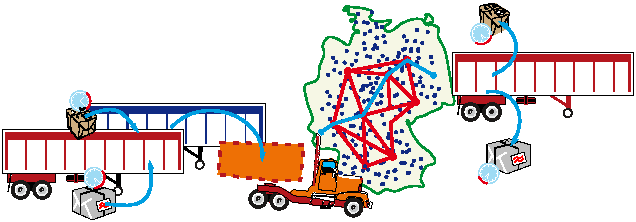
\includegraphics[width=0.99\linewidth]{\currentDir/logistic_planning}%
\caption{Illustrative sketch of logistics problems: Orders require us to pick up some items at source locations within certain time windows and deliver them to their destination locations, again within certain time windows. We need to decide which containers and vehicles to use and over which routes we should channel the vehicles.}
\label{fig:logistic_planning}
\end{figure}

The company could have the goals to fulfill all transportation requests \emph{at the lowest cost}.
Actually, it might seek to maximize its profit, which could even mean to outsource some tasks to other companies.
The goal of optimization then would be to find the assignment of containers to delivery orders and vehicles and of vehicles to routes, which maximizes the profit.
And it should do so within a limited, feasible time.

\begin{figure}%
\centering%
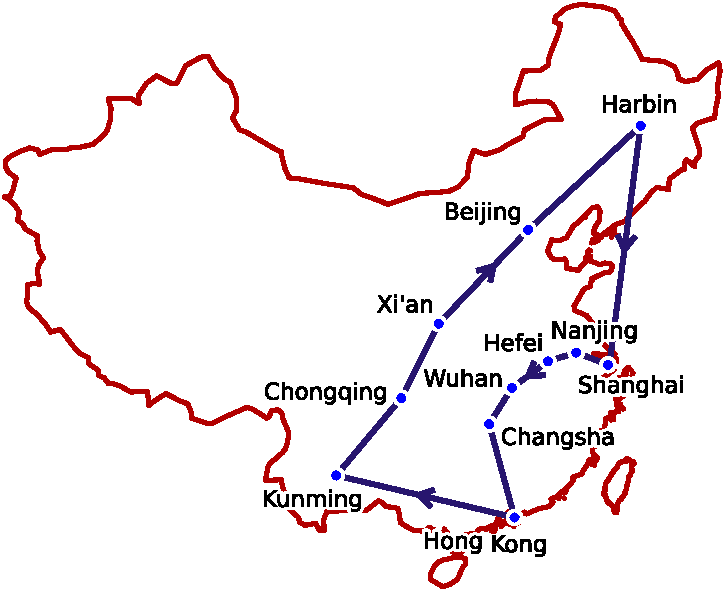
\includegraphics[width=0.6\linewidth]{\currentDir/tsp_china}%
\caption{A Traveling Salesperson Problem (TSP) through eleven cities in China.}%
\label{fig:tsp_china}%
\end{figure}%
%
Of course, there is a wide variety of possible logistics planning tasks.
Besides our real-world example above, a classical task is the Traveling Salesperson Problem~(TSP)~\cite{ABCC2006TTSPACS,LLRKS1985TTSPAGTOCO,GP2002TTSPAIV}, where the goal is to find the shortest round-trip tour through $n$~cities, as sketched in \autoref{fig:tsp_china}.
Many other scenarios can be modeled as such logistics questions, too:
If a robot arm needs to several drill holes into a circuit board, finding the shortest tour means solving a TSP and will speed up the production process, for instance~\cite{GJR1991OCOPADMACS}.%
\endhsection%
%
